\section*{Part 3 [68 points]}

\begin{enumerate}

    % PART 1
    \item \textbf{[34 points]} Describe and analyze your hand-crafted policy. 
    \begin{enumerate}



    % QUESTION b
    \item \textbf{[17 points]} With your scheduling policy, run the entire workflow \textbf{\textcolor{red}{3 separate times}}. For each run, measure the execution time of each batch job, as well as the latency outputs of memcached, running with a steady client load of 30K QPS. For each batch application, compute the mean and standard deviation of the execution time \footnote{Here, you should only consider the runtime, excluding time spans during which the container is paused.} across three runs. Also, compute the mean and standard deviation of the total time to complete all jobs - the makespan of all jobs. Fill in the table below. Finally, compute the SLO violation ratio for memcached for the three runs; the number of data points with 95th percentile latency $>$ 1ms, as a fraction of the total number of data points. The SLO violation ratio should be calculated during the time from when the first batch-job-container starts running to when the last batch-job-container stops running.  \\

    \begin{table}[ht]
        \centering
        \begin{tabular}{ |c|c|c|c|c|}
            \hline
            job name & mean time [s] & std [s] \\ \hline \hline
            \coloredcell{barnes}          & 63.33  & 1.53  \\  \hline
            \coloredcell{blackscholes}    & 47.67  & 3.06  \\  \hline
            \coloredcell{canneal}         & 107.33 & 1.53  \\  \hline
            \coloredcell{freqmine}        & 67.33  & 0.58  \\  \hline
            \coloredcell{radix}           & 20.67  & 2.08  \\  \hline
            \coloredcell{streamcluster}   & 113.33 & 16.20 \\  \hline
            \coloredcell{vips}            & 21.33  & 1.53  \\  \hline
            total time                    & 232.33 & 3.06  \\  \hline
        \end{tabular}
    \end{table}

    \textbf{Answer:}
    The memcached 95th percentile latency stayed well below the 1\,ms SLO during every run. Restricted to the window between the start of the first batch container and the completion of the last batch container (233\,s, 235\,s and 229\,s for runs 1--3), the mcperf output contains 21, 21 and 20 samples respectively, none of which exceeded 1\,ms; the highest observed p95 values were 378.6\,$\mu$s, 384.8\,$\mu$s and 375.2\,$\mu$s. The SLO violation ratio is therefore $0/21$, $0/21$ and $0/20$, i.e.\ \textbf{0\%} for all three runs.
    \\

    Create 3 bar plots (one for each run) of memcached p95 latency (y-axis) over time (x-axis), with annotations showing when each batch job started and ended, also indicating the machine each of them is running on. Using the augmented version of mcperf, you get two additional columns in the output: \texttt{ts\_start} and \texttt{ts\_end}. Use them to determine the width of each bar in the bar plot, while the height should represent the p95 latency. Align the $x$ axis so that $x=0$ coincides with the starting time of the first container.
    For each core in each machine show what job it is running using the colors proposed in this template (you can find them in \texttt{main.tex}). For example, draw a bar in {\color{vips}the color of vips} for core x from when vips is started to when it ends if vips ran on core x.
    %Use  the colors proposed in this template (you can find them in \texttt{main.tex}). For example, use the \colored{vips} color to annotate when vips started and stopped, the \colored{blackscholes} color to annotate when blackscholes started and stopped etc.

    \textbf{Plots:}
    \begin{figure}[H]
        \centering
        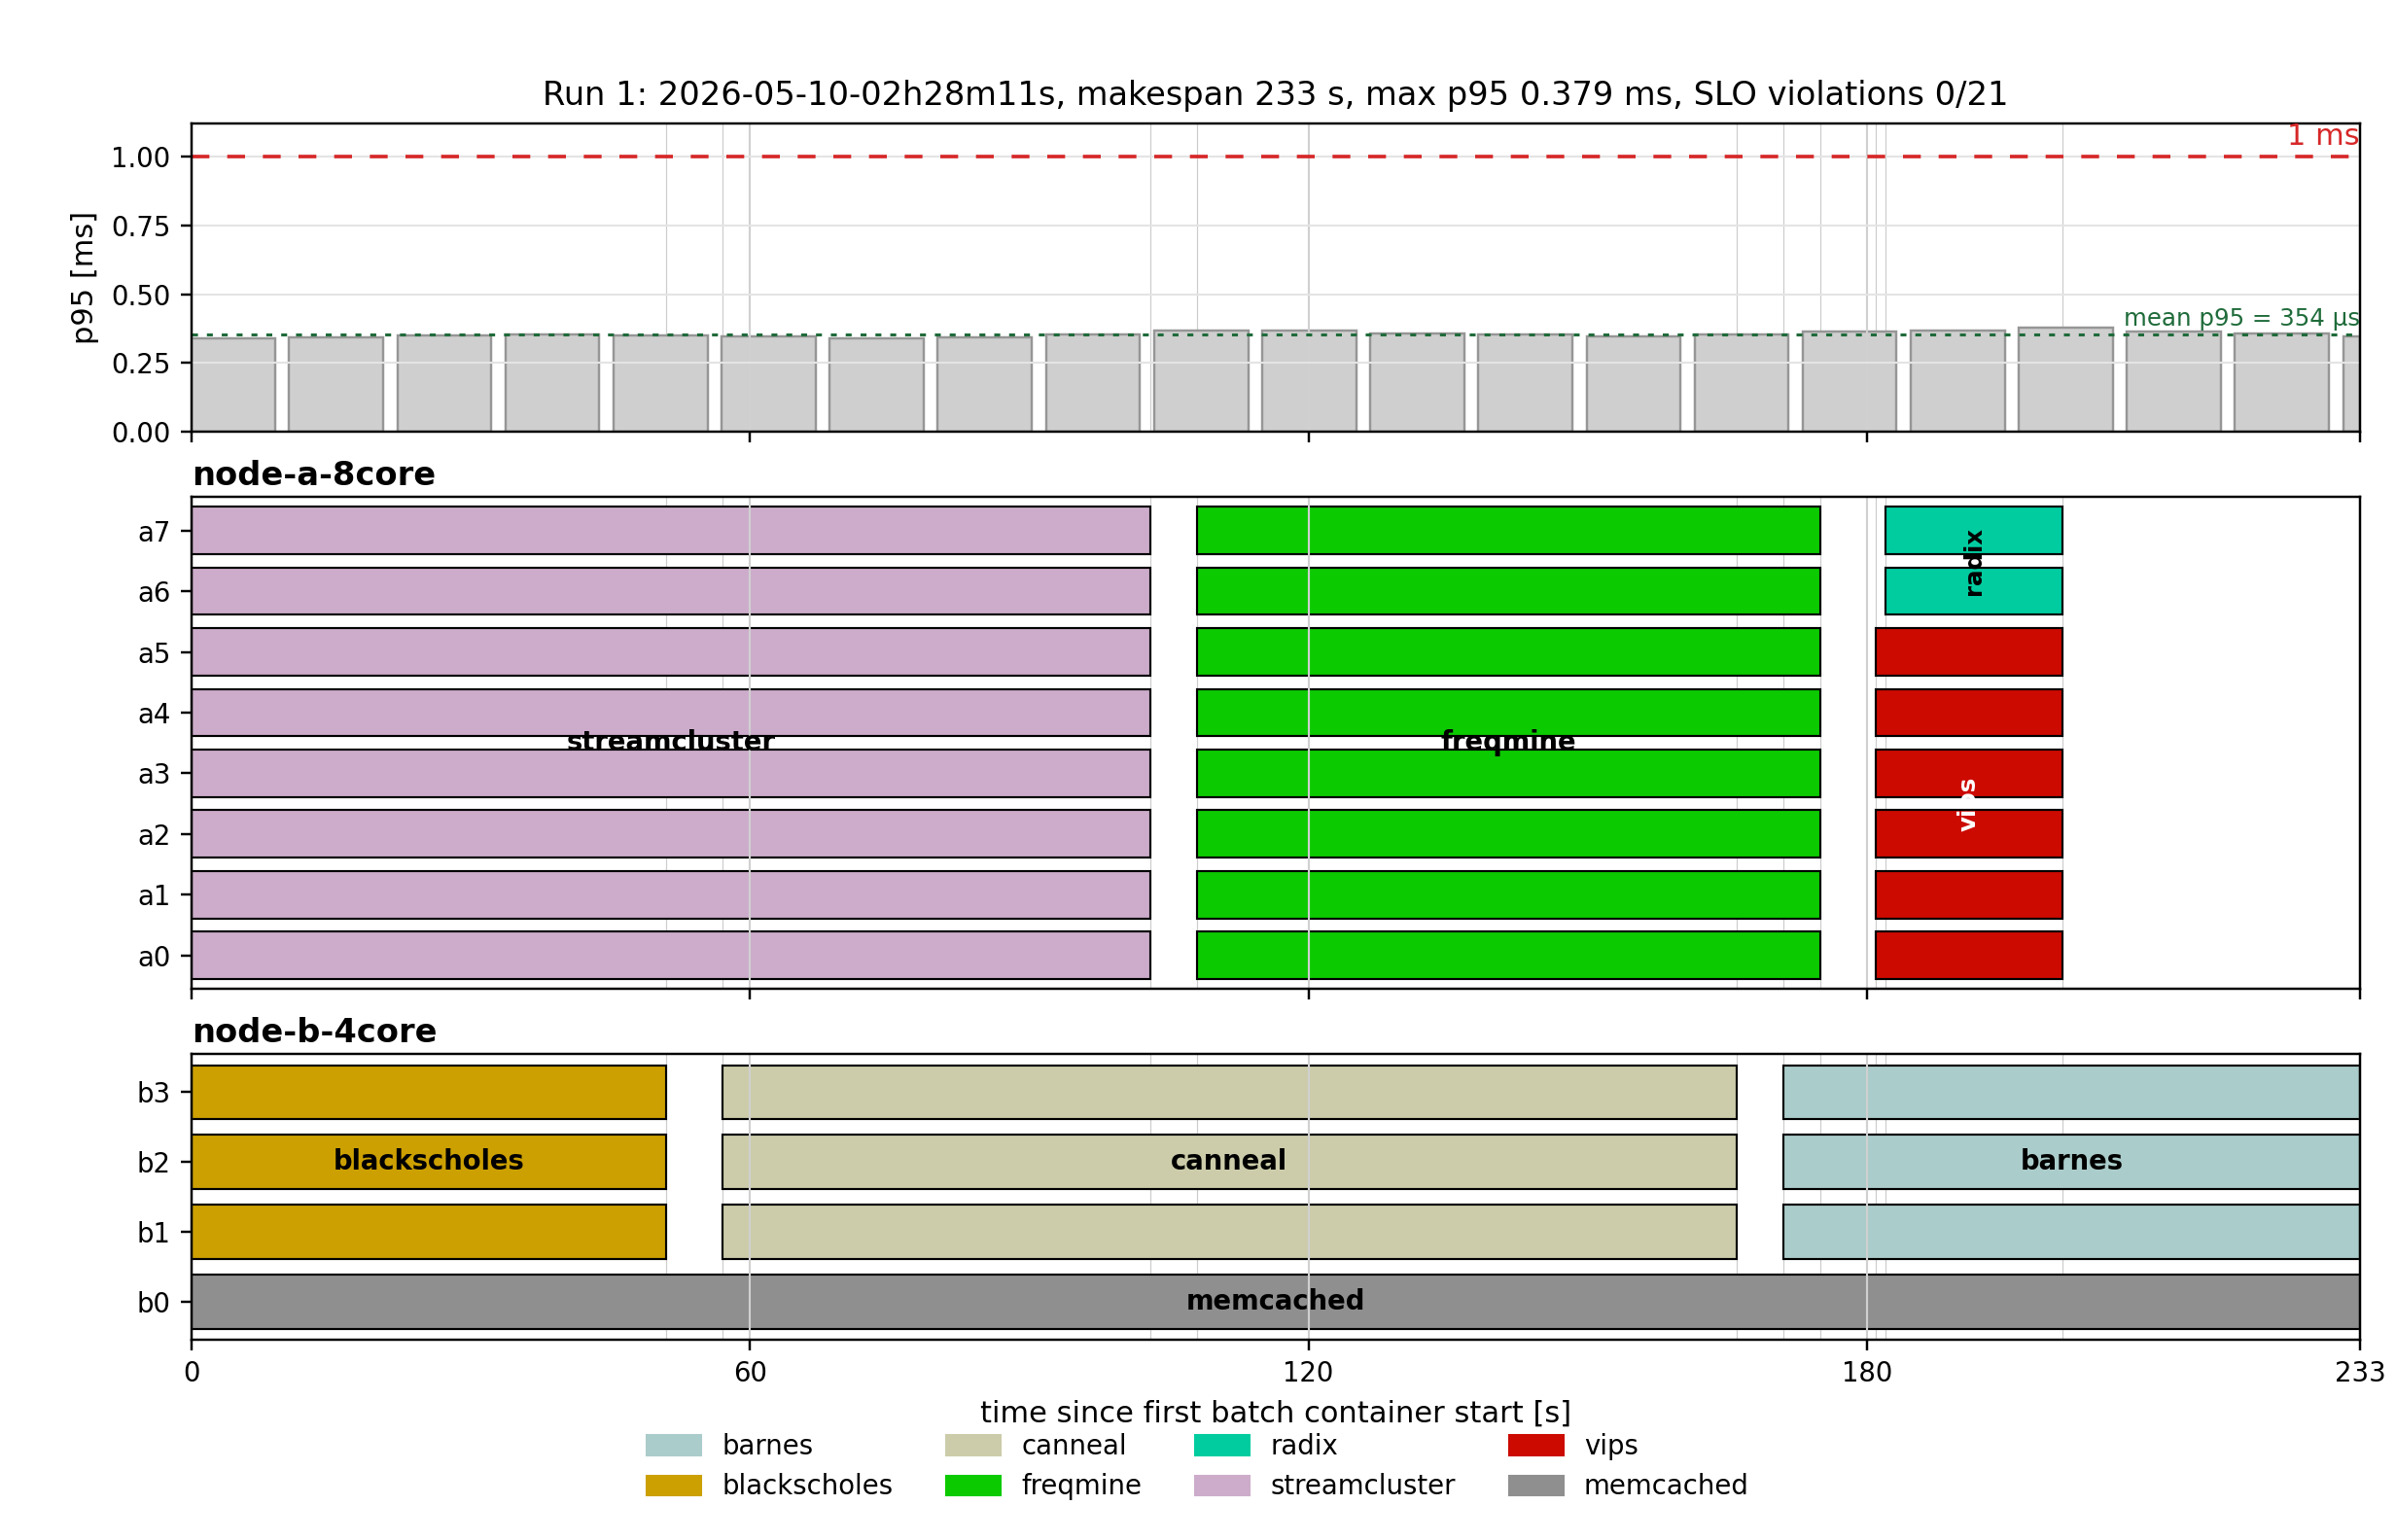
\includegraphics[width=\linewidth]{figures/cl_part3_q1a_run1.png}
        \caption{Run~1. Top: memcached p95 latency per 10\,s mcperf sample; the dashed red line marks the 1\,ms SLO. Bottom: per-core occupancy on \texttt{node-a-8core} and \texttt{node-b-4core}, coloured by batch job. Makespan = 233\,s, max p95 = 378.6\,$\mu$s, $0/21$ SLO violations.}
    \end{figure}
    \begin{figure}[H]
        \centering
        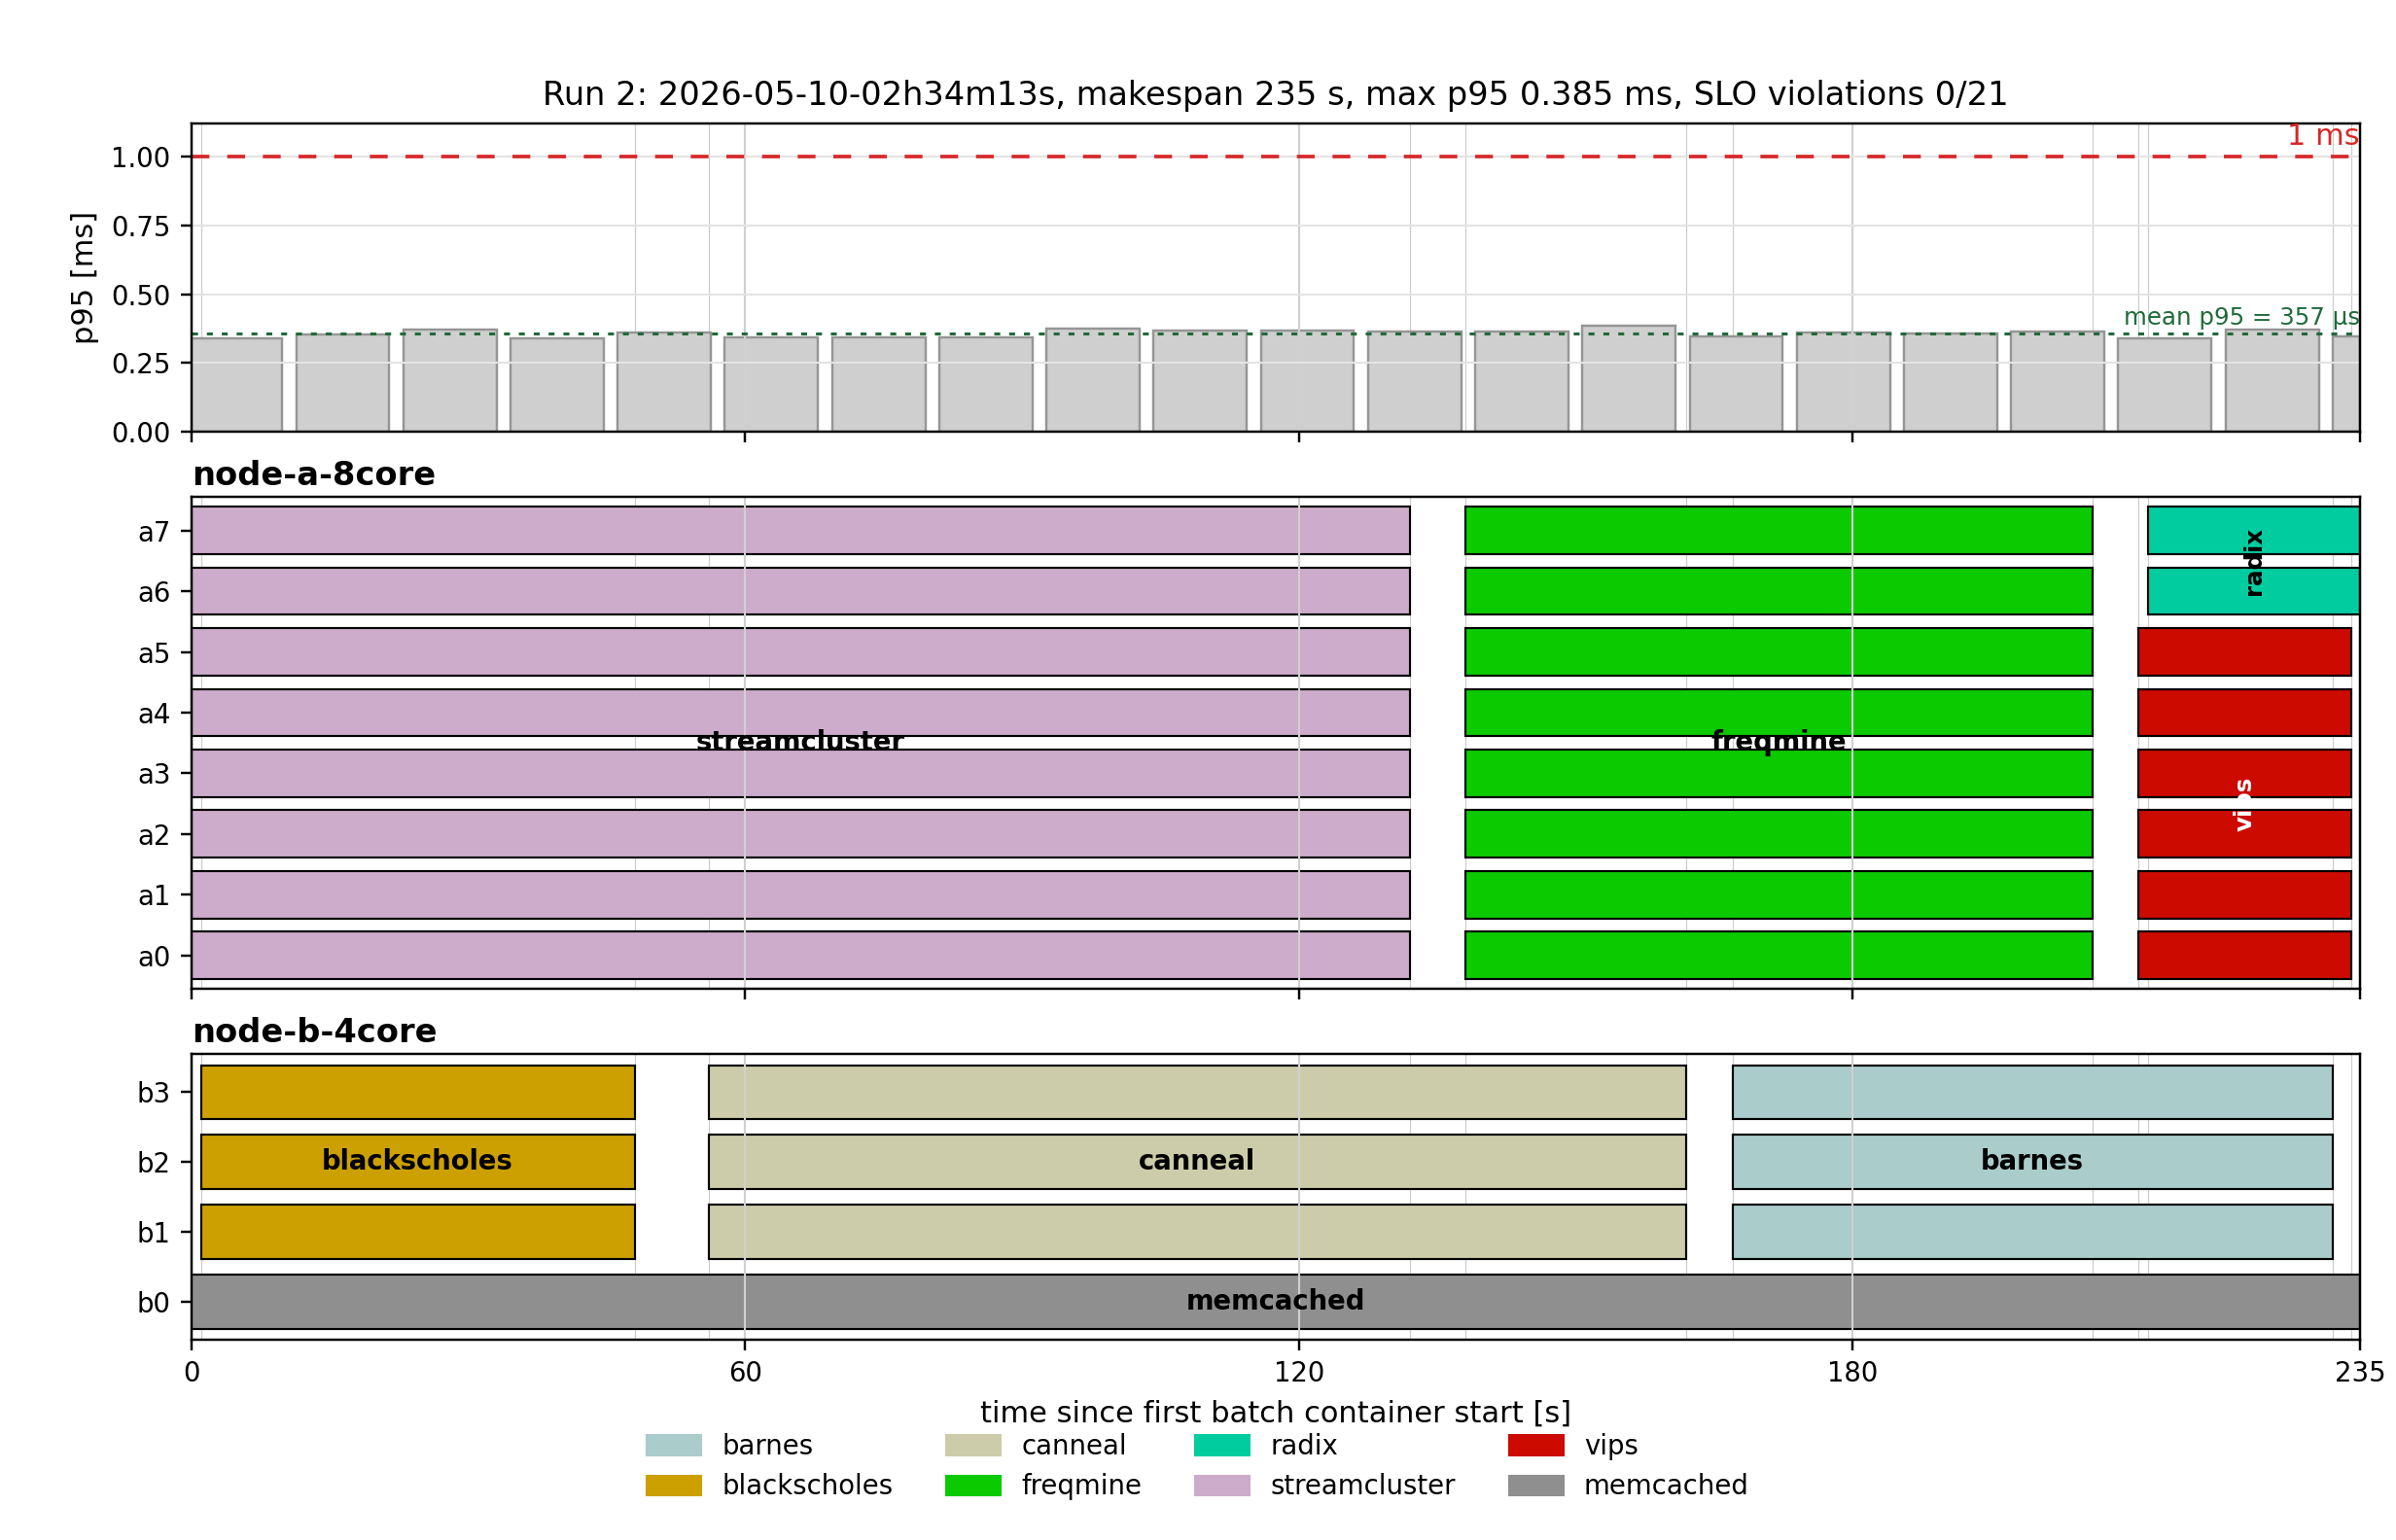
\includegraphics[width=\linewidth]{figures/cl_part3_q1a_run2.png}
        \caption{Run~2. Same layout as Run~1. Makespan = 235\,s, max p95 = 384.8\,$\mu$s, $0/21$ SLO violations.}
    \end{figure}
    \begin{figure}[H]
        \centering
        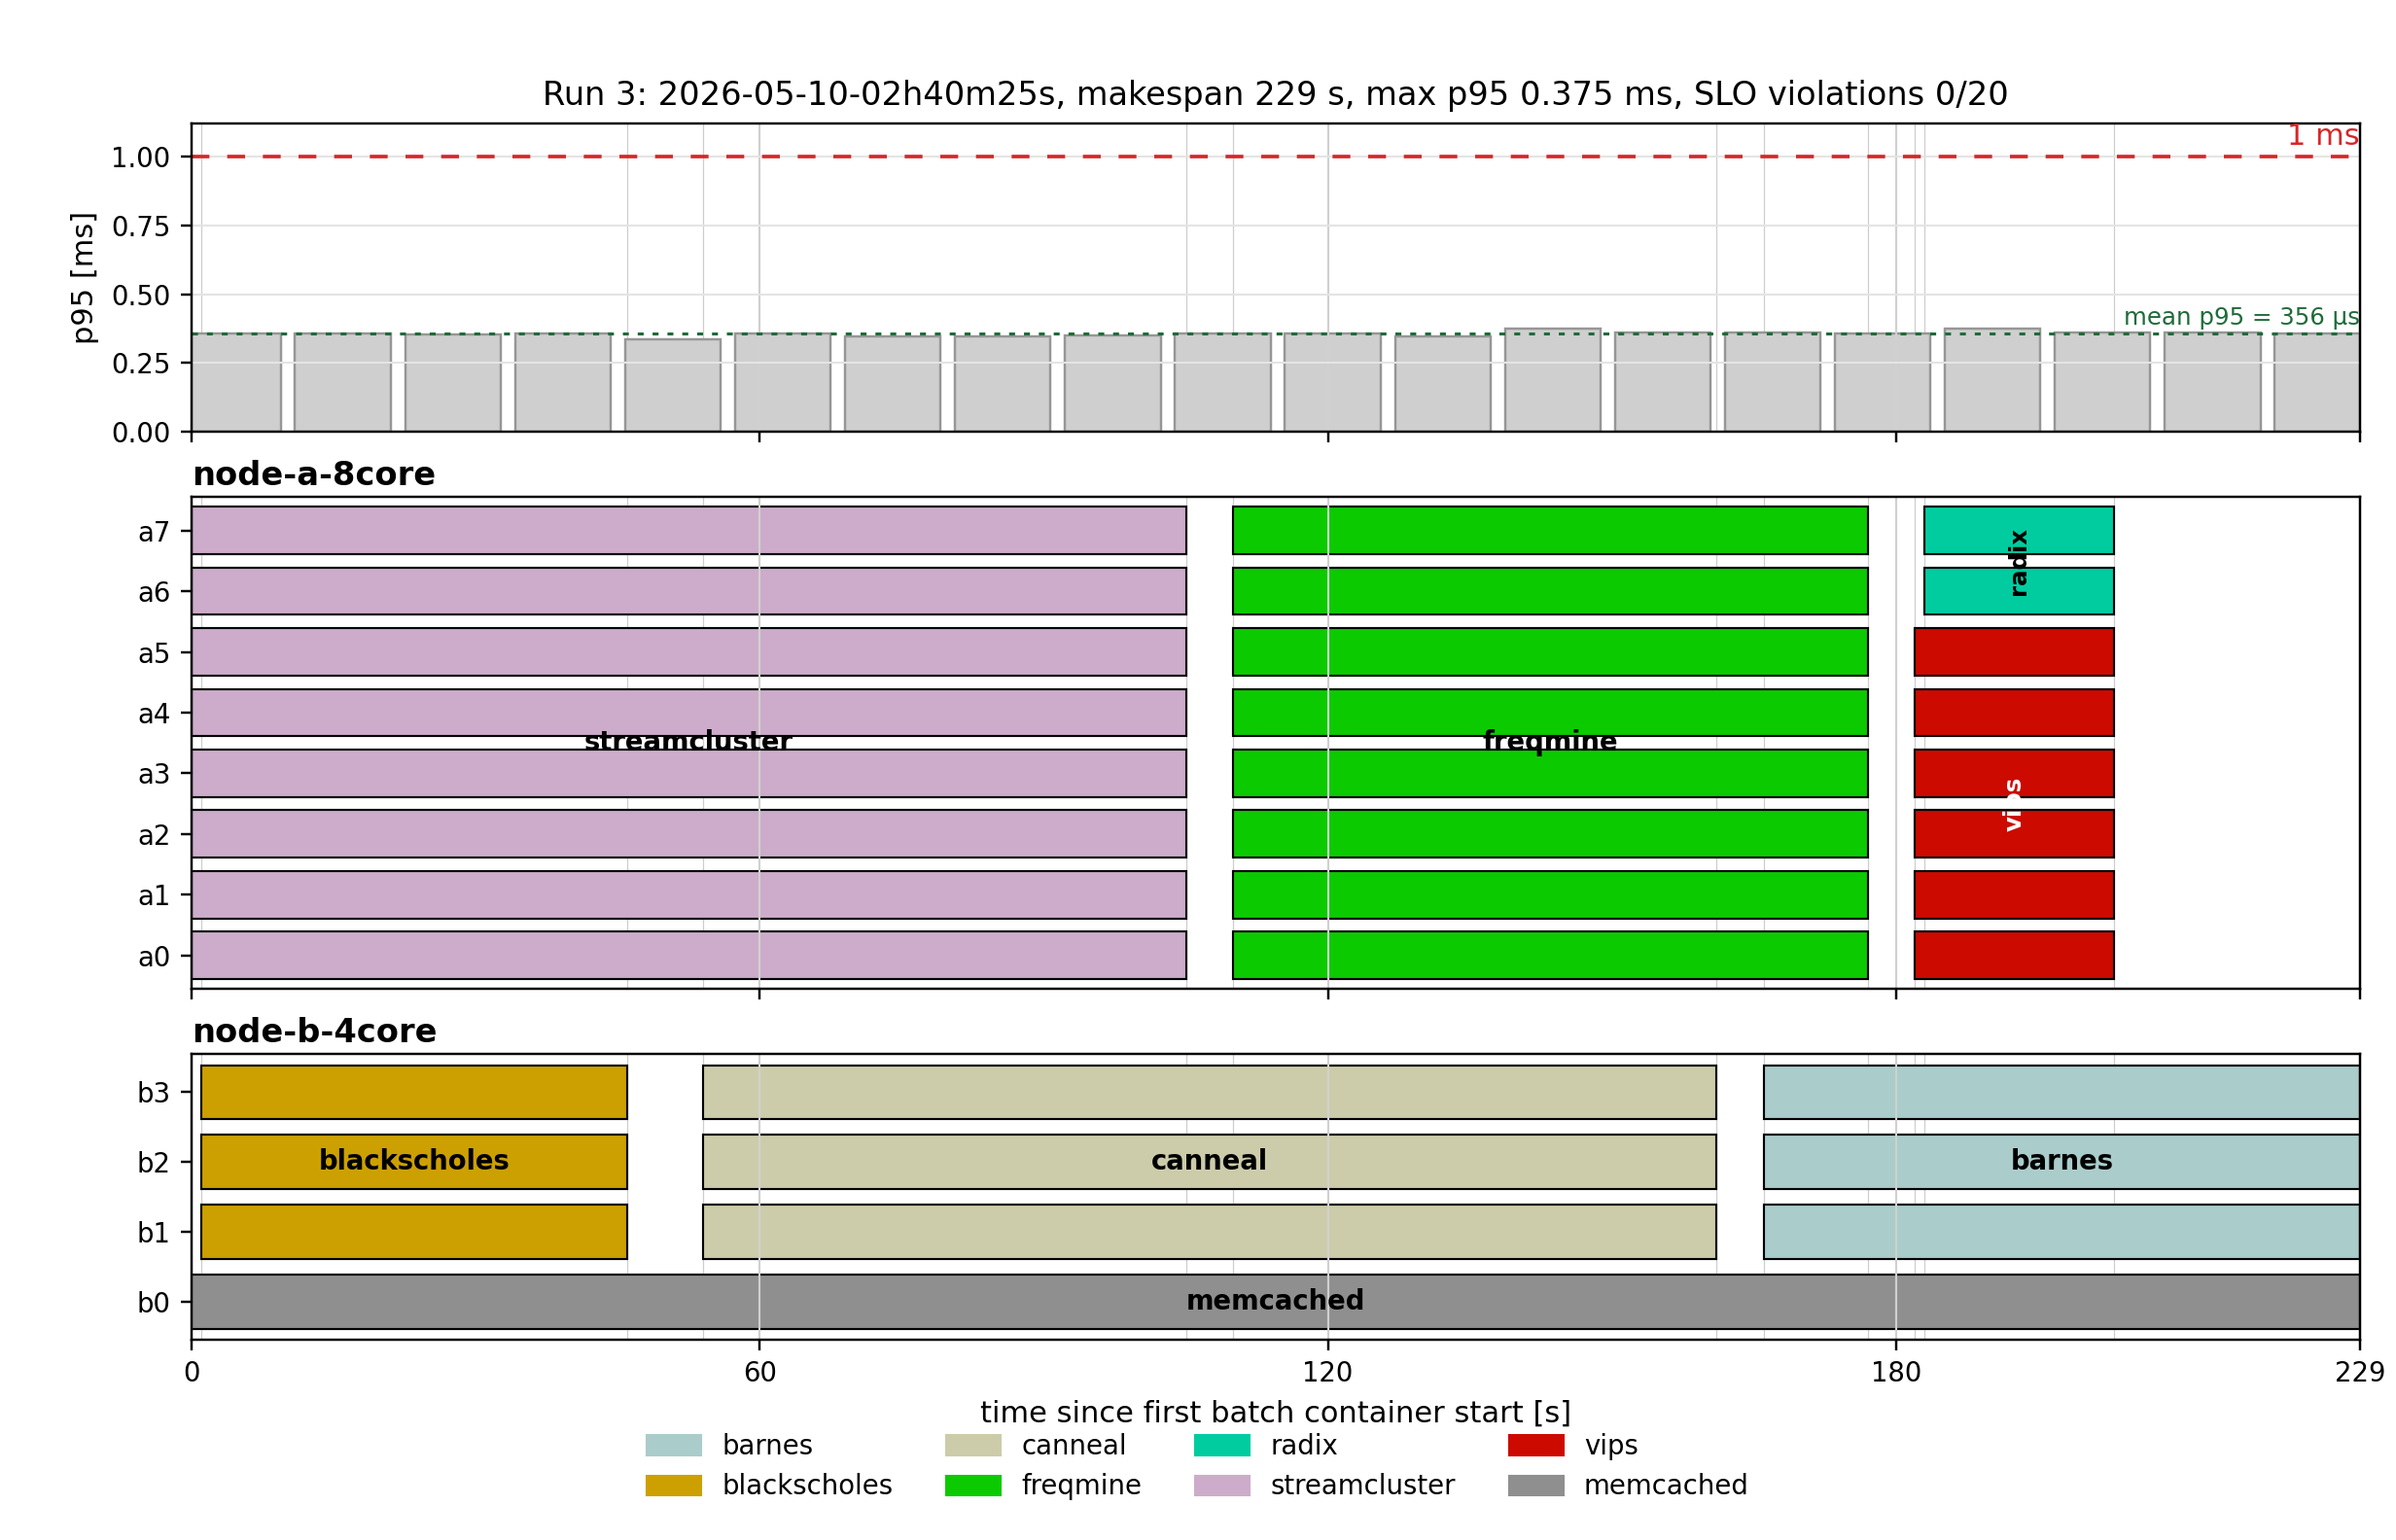
\includegraphics[width=\linewidth]{figures/cl_part3_q1a_run3.png}
        \caption{Run~3. Same layout as Run~1. Makespan = 229\,s, max p95 = 375.2\,$\mu$s, $0/20$ SLO violations.}
    \end{figure}


    % QUESTION b
    \item \textbf{[17 points]} Describe and justify the “optimal” scheduling policy you have designed. 
    
    \begin{itemize}
        \item Which node does memcached run on? Why?

        \textbf{Answer:}
        Memcached is pinned to a single core (core~0) of \texttt{node-b-4core}, the \texttt{n2d-highcpu-4} VM. The reasoning is multifaceted, and stems from a careful analysis of the physical properties of the hardware available to us. The two VMs requested in \texttt{part3.yaml} have very different shapes. The 8-core machine is an \texttt{e2-standard-8}, which on Google Cloud has an unpredictable CPU allocation that can land on slower Intel CPUs or a faster AMD Rome; in our experimentation the captured logs always reported an AMD Rome assignment. The 4-core machine is an \texttt{n2d-highcpu-4}, backed by either AMD Rome or AMD Milan (we were consistently assigned AMD Milan). The most important property is however the memory density: the \texttt{highcpu} shape provides only 1\,GB of RAM per core (4\,GB total on \texttt{node-b}), while the standard \texttt{e2} shape provides 4\,GB per core (32\,GB total on \texttt{node-a}).

        Given this asymmetry, placing memcached on the small node is the natural choice. From Part~1 we established that memcached is \emph{cache-bound, not DRAM-bound}: \texttt{ibench-membw} was the only interference source that left the SLO essentially intact, because memcached's working set fits in the LLC and rarely touches DRAM. Memcached therefore does not benefit from the larger memory pool of \texttt{node-a}, and putting it on the 4-core node frees the entire 8-core machine for the batch jobs that genuinely benefit from a high core count. Pinning memcached to core~0 of \texttt{node-b} also leaves the remaining three cores of that node free to host other batch jobs, which can be filled with workloads that are more DRAM-access bound (so that memcached's lack of DRAM pressure complements them rather than fighting them). During policy exploration we explicitly verified that this configuration does not trigger out-of-memory errors when batch jobs run on the same node as memcached, which was the main empirical risk associated with the small RAM budget of \texttt{node-b}.
        \\

        \item Which node does each of the 7 batch jobs run on? Why?

        \textbf{Answer:}
        The general principle, derived from Part~2, is that jobs which gain a large speedup going from 4 to 8 threads belong on \texttt{node-a-8core}, while jobs whose scaling plateaus around 4 threads (or whose working set is memory-intensive enough to make them good neighbours for memcached) belong on \texttt{node-b-4core}, where only 3 cores are available alongside memcached.

        \begin{itemize}
            \item \colored{barnes}: runs on \texttt{node-b-4core} (cores~1--3). Barnes scales well to 8 threads in isolation ($5.53\times$ in Part~2), but it is also strongly LLC-sensitive ($2.35\times$ slowdown under \texttt{ibench-llc}). Running it on \texttt{node-b} at the very end of the schedule, after \texttt{canneal} has finished, lets it run on a quiet machine: memcached is on a single private core and no other batch job is competing for the shared LLC.

            \item \colored{blackscholes}: runs on \texttt{node-b-4core} (cores~1--3). Part~2 showed that blackscholes plateaus completely between 4 and 8 threads ($2.36\times$ in both cases), indicating a memory-bandwidth bottleneck once the dataset is divided. Giving it 8 cores on \texttt{node-a} would therefore be wasteful, and \texttt{node-b} with 3 cores is a much better fit.

            \item \colored{canneal}: runs on \texttt{node-b-4core} (cores~1--3). Canneal scales poorly ($2.62\times$ at 8 threads, $1.57\times$ at 4) because of false sharing on the shared netlist, so the marginal value of placing it on the 8-core machine is small. Co-locating it with memcached is acceptable because memcached's working set lives in the LLC and is not on the critical path for canneal's random DRAM accesses.

            \item \colored{freqmine}: runs on \texttt{node-a-8core} (cores~0--7). Freqmine shows a strong non-monotonic improvement from 4 to 8 threads ($2.50\times \rightarrow 4.78\times$, an almost $2\times$ jump), so it is one of the jobs that benefits the most from having a full 8-core machine to itself.

            \item \colored{radix}: runs on \texttt{node-a-8core} (cores~6--7). Radix has good 4-to-8 scaling ($3.84\times \rightarrow 5.41\times$), but its total runtime is short (about 20\,s), so its wall-clock time is bounded by the container spin-up cost (approximately 6\,s with cached images) rather than by parallel speedup. Once this floor is taken into account, giving it just 2 cores at the tail of the schedule and letting it run in parallel with \texttt{vips} on the same node is more efficient than monopolising 8 cores for a short burst.

            \item \colored{streamcluster}: runs on \texttt{node-a-8core} (cores~0--7). Streamcluster has the best scaling of the entire suite ($5.80\times$ at 8 threads, $72\%$ parallel efficiency) and the longest runtime, so it is the prime candidate for the 8-core machine and is launched first to define the makespan on that side.

            \item \colored{vips}: runs on \texttt{node-a-8core} (cores~0--5). Vips scales well up to 4 threads ($3.85\times$) with diminishing returns at 8 ($4.60\times$), and it benefits from being on the AMD Rome platform of \texttt{node-a}. Running it on 6 cores in parallel with radix on the remaining 2 cores keeps the 8-core node fully utilised at the end of the schedule.
            \\

        \end{itemize}

        \item Which jobs run concurrently / are colocated? Why?

        \textbf{Answer:}
        The schedule produces three concurrent waves, one on each node, with the two nodes always running in parallel:
        \begin{itemize}
            \item \textbf{Wave~1} (start): \colored{streamcluster} on \texttt{node-a-8core} (8 threads) in parallel with \colored{blackscholes} on \texttt{node-b-4core} (3 threads). Streamcluster is the longest job with the best 8-thread scaling and therefore anchors the 8-core machine, while blackscholes saturates the 3 available cores on \texttt{node-b} without contending for memcached's core.
            \item \textbf{Wave~2}: \colored{freqmine} on \texttt{node-a-8core} (8 threads) in parallel with \colored{canneal} on \texttt{node-b-4core} (3 threads). Freqmine takes over the full 8-core node once streamcluster ends; canneal is the longest of the \texttt{node-b} jobs and is started as soon as blackscholes frees its cores.
            \item \textbf{Wave~3}: \colored{vips} (6 threads) and \colored{radix} (2 threads) share \texttt{node-a-8core}, while \colored{barnes} (3 threads) runs on \texttt{node-b-4core}. Vips and radix are co-located on the same node but on disjoint core sets, so they do not perform any simultaneous multithreading and do not compete for the same private caches. Splitting cores rather than serialising them is justified because both jobs are short enough that their wall-clock time is partly bounded by the container spin-up cost; running them in parallel on the same node hides one spin-up entirely.
        \end{itemize}
        Across all three waves, the only job ever co-located with memcached on \texttt{node-b} is the batch job currently scheduled there (blackscholes, then canneal, then barnes). This co-location is safe because memcached uses a dedicated private core (core~0), the batch job is confined to cores~1--3, and memcached's working set fits in the LLC, so the only shared resources are the LLC and the DRAM controller, both of which memcached barely exercises.
        \\

        \item In which order did you run the 7 batch jobs? Why?

        \textbf{Order}: \colored{streamcluster}, \colored{blackscholes} (both at \texttt{start}); \colored{freqmine} (after streamcluster), \colored{canneal} (after blackscholes); \colored{vips} and \colored{radix} (after freqmine), \colored{barnes} (after canneal).

        \textbf{Why}: The ordering follows a longest-job-first strategy, applied independently on each node, with the goal of equalising the finish times of the two nodes and keeping the 8-core machine continuously utilised. On \texttt{node-a-8core} the chain is \texttt{streamcluster} $\rightarrow$ \texttt{freqmine} $\rightarrow$ \texttt{(vips $\parallel$ radix)}, ordered by descending mean runtime among the jobs that benefit most from 8 threads. On \texttt{node-b-4core} the chain is \texttt{blackscholes} $\rightarrow$ \texttt{canneal} $\rightarrow$ \texttt{barnes}; \texttt{canneal} is the longest of the three and is placed in the middle so that it overlaps with the longer \texttt{freqmine} on \texttt{node-a} rather than running last and stretching the makespan. The two short, well-scaling jobs (\texttt{vips} and \texttt{radix}) are deliberately placed at the tail of the \texttt{node-a} chain and split across disjoint cores: their absolute runtime is so close to the container spin-up cost that running them sequentially would amount to paying the spin-up twice for no parallel benefit. As a worked example, two jobs whose isolated runtimes are 20\,s on 4 cores and 10\,s on 8 cores would take $6 + 10 + 6 + 10 = 32$\,s if executed sequentially on 8 cores, versus $6 + 20 = 26$\,s if executed in parallel on 4 cores each; this 6\,s spin-up floor is why we precache the container images before each run and why we co-locate \texttt{vips} and \texttt{radix} on disjoint cores at the end.
        \\

        \item How many threads have you used for each of the 7 batch jobs? Why?

        \textbf{Answer:}
        The general rule we enforced is that the thread count of a job equals the number of cores it is assigned, never more. We deliberately did not explore policies that oversubscribe a core or rely on simultaneous multithreading. This rule was motivated both by simplicity (it dramatically reduces the search space of admissible policies) and by the empirical evidence from Parts~1 and~2: the dominant source of latency degradation in our measurements was L1d/L1i/L2/LLC misses, all of which are aggravated when two threads share the same physical core.

        \begin{itemize}
            \item \colored{barnes}: 3 threads on cores~1--3 of \texttt{node-b-4core}. Barnes scales well, but the 4-core node only offers 3 free cores once memcached takes core~0.

            \item \colored{blackscholes}: 3 threads on cores~1--3 of \texttt{node-b-4core}. Part~2 showed that blackscholes does not benefit from going beyond 4 threads, so 3 threads is essentially on the plateau of its speedup curve and no throughput is lost by giving it the smaller node.

            \item \colored{canneal}: 3 threads on cores~1--3 of \texttt{node-b-4core}. Canneal's parallel efficiency is poor ($33\%$ at 8 threads in Part~2), so 3 threads on \texttt{node-b} extracts most of the realistic speedup while leaving the 8-core node for jobs that scale better.

            \item \colored{freqmine}: 8 threads on cores~0--7 of \texttt{node-a-8core}. Freqmine almost doubles its speedup between 4 and 8 threads, so it is one of the jobs that most justifies the use of the full 8-core machine.

            \item \colored{radix}: 2 threads on cores~6--7 of \texttt{node-a-8core}. Radix scales well in isolation, but at $\sim$20\,s of runtime its wall-clock time is close to the container spin-up floor; 2 threads is enough to finish before vips (running on the other 6 cores of the same node) does, and using fewer cores frees the rest of the node for vips.

            \item \colored{streamcluster}: 8 threads on cores~0--7 of \texttt{node-a-8core}. Streamcluster has the best scaling in the suite ($5.80\times$, $72\%$ efficiency), so it receives the full 8-core machine for its entire duration.

            \item \colored{vips}: 6 threads on cores~0--5 of \texttt{node-a-8core}. Vips shows diminishing returns past 4 threads, so a 6-core allocation captures most of the available speedup while leaving 2 cores for radix to run in parallel on the same node.
            \\
        \end{itemize}

        \item Which files did you modify or add and in what way? Which Kubernetes features did you use?

        \textbf{Answer:} A detailed description of the modified files, the automation scripts, and the Kubernetes features used is deferred to the corresponding question below, where the full coordination pipeline, the precaching pod, the policy validator, the resource-contention checker and the web visualisation tool are discussed together.
        \\

        \item Describe the design choices, ideas and trade-offs you took into account while creating your scheduler (\underline{if not already mentioned above}). Describe how your policy (and its performance) compares to another policy that you experimented with (in particular to the second-best policy that you designed).

        \textbf{Answer:}
        Beyond the per-node, per-job and ordering decisions justified above, three further design choices shaped our final policy.

        First, we explicitly excluded any form of simultaneous multithreading or core oversubscription from the search space. No two jobs were ever scheduled on the same physical core, and no job was ever given a thread count higher than its assigned core count. The motivation was twofold: it sharply reduces the combinatorial space of admissible policies, and it is also consistent with the bottleneck analysis from Parts~1 and~2, which identified L1d/L1i/L2/LLC pressure as the dominant source of latency degradation for memcached and of slowdown for the batch jobs. Allowing two threads to share a core would have re-introduced exactly the kind of cache pollution that those parts already characterised as the worst-case interference.

        Second, container spin-up time emerged from our empirical runs as a non-negligible metric, of the order of 6\,s per container even when the image is already cached on the node. For short jobs with high parallel scaling (in our case \texttt{radix} and \texttt{vips}) this floor is large enough to invert the apparent winner between sequential execution on more cores and parallel execution on fewer cores. To mitigate this we added a small precaching pod to the deployment pipeline that pulls every required image on both nodes before the benchmark suite runs, and we also redesigned the tail of the schedule so that \texttt{vips} and \texttt{radix} run concurrently on disjoint cores of \texttt{node-a} rather than back-to-back on all eight cores.

        Third, the policy is the result of an exploration in which we used the running statistics of past runs (job durations, observed memcached p95) as a guide. Earlier candidate policies tried to keep \texttt{barnes} on \texttt{node-a} (because of its good 8-thread scaling) and to put one of the short \texttt{node-a} jobs on \texttt{node-b}; the resulting makespan was slightly worse because \texttt{barnes} is also strongly LLC-sensitive, and on a busy \texttt{node-a} it actually ran more slowly than on a quiet \texttt{node-b} at the tail of the schedule. Our second-best policy left \texttt{vips} and \texttt{radix} serialised on the full 8-core node instead of co-locating them on disjoint cores; this preserved per-job speedup but paid the container spin-up cost twice and produced makespans roughly 10--15\,s longer than the final design, while never improving the SLO violation ratio (which remained at $0\%$ for both policies).
        \\


    \end{itemize}
    \end{enumerate}


    % PART 2
    \item \textbf{[34 points]} Describe and analyze the AI-generated policy. [TODO: Xiaozhe]

    \begin{enumerate}

        % QUESTION a
        \item \textbf{[17 points]} \textbf{Report the performance}:
        
        \begin{itemize}
            \item Report the mean time of each batch job, as well as the makespan of all jobs for the AI-generated policy. Also, report the SLO violation ratio for memcached for the AI-generated policy. \textit{Note: If the LLM failed to produce a valid solution after 3+ attempts, provide the error logs and your best-performing manual tweak for partial credit.}
        
        \begin{table}[ht]
            \centering
            \begin{tabular}{ |c|c|c|c|c|} 
                \hline
                job name & mean time [s] (Baseline) & mean time [s] (AI) \\ \hline \hline
                \coloredcell{barnes}          & & \\  \hline
                \coloredcell{blackscholes}    & & \\  \hline
                \coloredcell{canneal}         & & \\  \hline
                \coloredcell{freqmine}        & & \\  \hline
                \coloredcell{radix}           & & \\  \hline
                \coloredcell{streamcluster}   & & \\  \hline
                \coloredcell{vips}            & & \\  \hline
                total time      & & \\  \hline
            \end{tabular}
        \end{table}

    \item Create 3 bar plots (one for each run), for the final AI-generated policy, of memcached p95 latency (y-axis) over time (x-axis), with annotations showing when each batch job started and ended, also indicating the machine each of them is running on. Use the same method as described in the previous question to create the bar plots.
    
    \textbf{Answer:}
    \item Create two line plots (one for the p95 latency and one for SLO violations) showing policy performance over iterations.
    
    \textbf{Answer:}
    \end{itemize}

    % QUESTION b
    \item \textbf{[17 points]} Analysis of the Evolutionary Process: Describe the process of how you used OpenEvolve to design the AI-generated policy. For example, you can include the following details in your answer (You are not limited to these questions. You can include any other details you find relevant and interesting). Your response will be graded based on the thoroughness of the exploration and clarity in explanation:
        
        \begin{itemize}
            \item How many iterations did you run through OpenEvolve with the LLMs to get to the final policy? Which LLM(s) did you use?
            \item How do you measure success? For example, how do you design the `combined\_score' or the success metric, given that there are two objectives (makespan and SLO violations)?
            \item Describe the initial policy you fed to the LLM(s) and why you chose this as the initial policy.
            \item Describe how the policy changes during the process, and how it impacted the performance of the policy (e.g., tail latency; SLO violations).
            \item Explain why did this AI-generated policy perform better (or worse) than the baseline?
            \item Identify one ``hallucination'' or logical flaw the model produced during the process and how you identified it.
        \end{itemize}

         \textbf{Answer:}


    \end{enumerate}

    Please attach your modified/added YAML files, run scripts, OpenEvolve scripts, experiment outputs and the report as a zip file. You can find more detailed instructions about the submission in the project description file.
    
    \textbf{Important: The search space of all possible policies is exponential and you do not have enough credits to run all of them. We do not ask you to find the policy that minimizes
    the total running time, but rather to design a policy that has a reasonable running time, does not violate the SLO, and takes into account the characteristics of the first two parts of the project.}
\end{enumerate}

\newpage
